For every \(p \in \R^{n+1}\) and \(\lambda>0\), let
\[
    \eta_{p,\lambda}(x) = \frac{x-p}{\lambda} \qquad \forall x \in \R^{n+1}.
\]

\begin{defn}
    A \emph{cone} in \(\R^{n+1}\) with vertex \(p \in \R^{n+1}\) is a subset \(C \subseteq \R^{n+1}\) such that
    \[
     \eta_{p,\lambda}(C)=\eta_{p,0}(C) \qquad \forall \lambda>0.
    \]
    The \emph{link} of a cone \(C\) is
    \[
        S=S(C) \coloneq C \cap \Sp^{n}(p),
    \]
    where \(\Sp^{n}(p)\) is the unit sphere centered at \(p\).
\end{defn}

From now on, unless explicitly specified, every cone is assumed to have vertex \(p=0\). For any \(r>0\), we will denote
\[
    C_r \colon \{ x \in C \colon 0<|x|<r \}, \qquad S_r = \{ x \in C \colon |x|=r\}.
\]

The \emph{regular set} \(\Reg(C)\) of the cone \(C\) is the maximal relatively open set \(M \subset C\) which is a smooth submanifold of \(\R^{n+1}\).The \emph{singular set} of \(C\) is \(\Sing(C) \coloneq C \setminus \Reg(C)\). A cone \(C\) is said to be \emph{regular} if \(\Sing(C) \subseteq \{p\}\).

\begin{rmk}
    If \(C \subset \R^{n+1}\) is a cone with link \(S\), then clearly
    \[
        C \setminus \{0\}= \bigcup_{v \in S}\{ tv \colon t>0 \}.
    \]
    Thus \(S\) is a smooth submanifold of \(\Sp^{n}\) if and only if \(C\) is a regular cone.
\end{rmk}

If \(\llbracket C \rrbracket\) is a stationary current, then \(\Reg(C)\) is a minimal hypersurface, as one can always take variations supported on \(\Reg(C)\). 

\subsection{Analysis of the Jacobi operator of a cone}
Let \(C \subset \R^{n+1}\) be an \(n\)-dimensional cone in the sense of currents (i.e., \(C\) is a current which is scale invariant). 

If \(r(x) = |x|\), then a simple computation is spherical coordinates show that on \(\Reg(C)\)
\begin{equation*}
    \begin{aligned}
        g_C &= \dif r^2 + r^2 g_S,\\
        A_C &= r^{-1}A_S, \\
        \Delta_C &= \frac{\de^2}{\de r^2} + \frac{n-1}{r} \frac{\de}{\de r} + \frac{1}{r^2} \Delta_S
    \end{aligned}
\end{equation*}
where \(A_S\) is the second fundamental form of (the regular part of) \(S\) in \(\Sp^n\). As a consequence:
\begin{prop}\label{prop: cone minimal iff link minimal}
    A regular cone \(C \subset \R^{n+1}\) is minimal if and only if its link \(S\) is a minimal submanifold of \(\Sp^{n}\).
\end{prop}

Let \(C \subset \R^{n+1}\) be a regular \(n\)-dimensional minimal cone (or also the regular part of a stationary cone, e.g. \(\mathcal{R}_{\ge \rho}(C)\) for some \(\rho>0\)). Its Jacobi operator is
\[
L_C = \frac{\de^2}{\de r^2} + \frac{n}{r} \frac{\de}{\de r} + \frac{1}{r^2} (\Delta_S +|A_S|^2).
\]
We will study independently the two operators
\[
    L = \Delta_S +|A_S|^2
\]
on the link and 
\[
    P=r^2 \frac{\dif^2}{\dif r^2} + (n-1)r \frac{\dif }{\dif r}
\]
on a segment, and then combine the obtained results. 

Consider \(L \coloneq \Delta_S + |A_S|^2\) on a relatively open subset \(\Omega\) of \(S\) with smooth (possibly empty, if \(S\) is smooth) boundary, and impose homogeneous Dirichlet conditions. By standard elliptic theory, it can be diagonalized, i.e., we can find a Hilbert basis \(\{\psi_j\}_{j \in \N}\) of \(C^\infty_0(\Omega)\) and a monotone sequence
\[
    \mu_1 \le \mu_2 \le \dots  \to \infty
\]
such that
\[
    -L\psi_j = \mu_j \psi_j.
\]
Moreover,
\begin{equation}\label{eq: variational eigenvalue}
    \mu_1 = \mu_1(\Omega) = \inf \left\{ \frac{\int_\Omega |\nabla u|^2- |A_S|^2u^2}{\int_\Omega u^2} \colon u \in C^\infty_c(\Omega) \setminus \{0\}\right\}.
\end{equation}

\begin{lemma}\label{lemma: 1st eigenvalue of minimal hypersurfaces in the sphere}
    Let \(S \subset \Sp^n\) be a closed (i.e. compact and without boundary) minimal hypersurface of the round \(n\)-sphere. If \(S\) is not a totally geodesic \((n-1)\)-sphere, then
    \[
        \mu_1(S) \le -(n-1).
    \]
\end{lemma}
\begin{proof}
    Test the function \(u= |A_S|\) (up to smoothing) and use Simons' identity \cite[Theorem~5.3.1]{Simons_MinimalVarieties1968}:
    \begin{equation}\label{eq: Simons identity}
        \Delta_S A_S = (n-1-|A_S|^2)A_S.
    \end{equation}

    Fix an orthonormal frame \(E_1,\dots,E_{n-1}\) tangent to \(S\). Observe that
    \[
        \nabla_X |A_S| = |A_S|^{-1}\langle \nabla_X A_S, A_S \rangle 
    \]
    for any \(X \in \VF(S)\), so
    \[
    \begin{split}
        \nabla_{E_i} (\nabla_{E_i}|A_S|) &= -|A_S|^{-3} \langle \nabla_{E_i} A_S, A_S \rangle^2 + |A_S|^{-1}(|\nabla_{E_i}A_S|^2+ \langle \nabla_{E_i} \nabla_{E_i} A_S, A_S \rangle ) \\
        \nabla_{\nabla_{E_i}E_i} |A_S| &= |A_S|^{-1}\langle \nabla_{\nabla_{E_i}E_i} A_S, A_S \rangle.
    \end{split}
    \]

    Then,
    \begin{align*}
        \Delta_S |A_S| &= \sum_i \nabla_{E_i} (\nabla_{E_i} A_S) - \sum_i \nabla_{\nabla_{E_i}E_i}A_S \\
        &= |A_S|^{-1} \sum_i \langle \nabla_{E_i}\nabla_{E_i} A_S - \nabla_{\nabla_{E_i}E_i} A_S, A_S \rangle \\
        &\qquad \qquad \qquad + |A_S|^{-1} \sum_i (|\nabla_{E_i}A_S|^2 - |A_S|^{-2}\langle\nabla_{E_i}A_S, A_S \rangle ^2 ).
    \end{align*}
    By Cauchy-Schwarz inequality,
    \begin{align*}
        |\nabla_{E_i}A_S|^2 - |A_S|^{-2}\langle\nabla_{E_i}A_S, A_S \rangle^2 &\ge |\nabla_{E_i}A_S|^2 - |\nabla_{E_i}A_S|^2 \ge 0.
    \end{align*}
    By \eqref{eq: Simons identity},
    \begin{align*}
        \Delta_S |A_S| &\ge |A_S|^{-1} \sum_i \langle \nabla_{E_i}\nabla_{E_i} A_S - \nabla_{\nabla_{E_i}E_i} A_S, A_S \rangle = |A_S|^{-1}{\langle \Delta A_S,A_S\rangle} \\
        &= (n-1-|A_S|^2)|A_S|.
    \end{align*}

    Testing \(u=|A_S|\) (up to smoothing) in \eqref{eq: variational eigenvalue} we get
    \begin{align*}
        \mu_1 &\le \frac{1}{\int_S |A_S|^2\dif \sigma}\int_S |\nabla_S |A_S||^2 \dif \sigma - \int_S |A_S|^4\dif \sigma \\
        &= -\frac{1}{\int_S |A_S|^2 \dif \sigma} \int_S |A_S| \Delta |A_S| +|A_S|^4 \dif \sigma \\
        &\le -\frac{1}{\int_S |A_S|^2 \dif \sigma} \int_S (n-1) |A_S|^2 \dif \sigma \\
        &= -(n-1). \qedhere
    \end{align*}
\end{proof}

\begin{rmk}\label{rmk: 1st eigenvalue on the link}
    If \(C\) is not regular, then there exists \(\rho_0>0\) such that
    \[
        \mu_1(\mathcal{R}_{\ge \rho_0}\cap \Sp^n) \le -(n-1).
    \]
    The idea is again to test \(u=|A_S|\), but of course one needs to be even more careful because \(|A_S|\) does not vanish at \(\de (\mathcal{R}_{\ge \rho_0}\cap \Sp^n)\). 
\end{rmk}

Let us now consider the differential operator
\[
    Pu (r)= r^2 u''(r) + (n-1)r u'(r).
\]
Given \(\mu \in \R\), we can find a general (complex) solution of 
\[
    Pu =\mu u
\]
by plugging the ansatz \(u(r)=r^\gamma\), getting that
\[
    \gamma^2+(n-2)\gamma =\mu
\]
so
\[
    \gamma = \gamma^\pm(\mu) = \frac{2-n}{2} \pm \sqrt{ \left(\frac{n-2}{2}\right)^2 + \mu}.
\]

    \begin{figure}[ht]
        \centering
        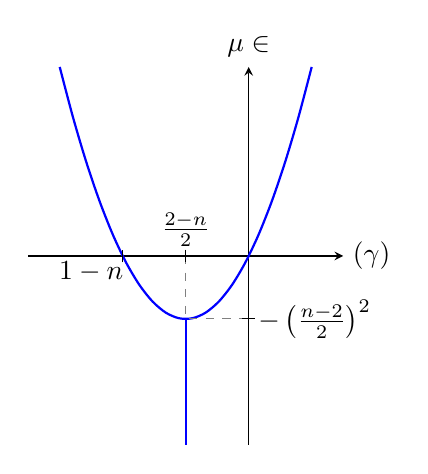
\begin{tikzpicture}[scale=0.8,>=stealth]
          % parameter
          \def\n{4}
          \pgfmathsetmacro{\m}{.5*(2-\n)}
          \pgfmathsetmacro{\t}{\m*\m+(\n-2)*\m}
          \pgfmathsetmacro{\z}{2-\n}
          \pgfmathsetmacro{\a}{\m-2}
          \pgfmathsetmacro{\b}{\m+2}
          \pgfmathsetmacro{\f}{\b*\b+(\n-2)*\b}
        
          % axes
          \draw[->] (\a-0.5,0) -- (\b+0.5,0) node[right] {$\re(\gamma)$};
          \draw[->] (0,\t-2) -- (0,\f) node[above] {$\mu \in \R$};
        
          % parabola: lambda = gamma^2 + (n-2)*gamma + 1 - n, gamma real
          \draw[domain=\a:\b,samples=20,smooth,thick,blue]
            plot(\x,{\x*\x + (\n-2)*\x});

          % real trace: re(gamma) = (n-2)/2
          \draw[thick, blue](\m,\t)--(\m,\t-2);

        
          % labels
          \draw (\z,-.1)--(\z,.1);
          \node at (\z-.5,-.25) {$1-n$};

          \draw[dashed,gray] (\m,0) -- (\m,\t)--(0,\t);
          \draw (\m,.1)--(\m,-.1);
          \draw (-.1,\t)--(.1,\t);
          \node[above] at (\m,0){\(\frac{2-n}{2}\)};
          \node[right] at (0,\t){\(-\left(\frac{n-2}{2}\right)^2\)};        
        \end{tikzpicture}
        \caption{In blue \(\{(\re(\gamma),\mu) \in \R^2 \colon\gamma^2+(n-2)\gamma = \mu\}\).}
        \label{fig: parabola}
    \end{figure}

Substituting \(v=r^{-\gamma}u\) with \(\gamma = \gamma^\pm(\mu)\), we find that
\[
   \left[r^{n-1+2\gamma}v' \right]' = 0.
\]
Thus \(v' = cr^{1-n-2\gamma}\), so the general solution of \(Pu=\mu u\) (in \(\C\)) is 
\begin{equation}\label{eq: general solution of u}
u(r)= \left\{
\begin{aligned}
    &c_1 r^{2-n-\gamma} + c_2 r^\gamma &&\gamma \ne \frac{2-n}{2} \iff \mu \ne - \left(\frac{n-2}{2}\right)^2 \\
    &c_1 r^{\frac{2-n}{2}}(\log r + c_2) && \gamma = \frac{2-n}{2} \iff \mu = - \left(\frac{n-2}{2}\right)^2.
\end{aligned}\right.
\end{equation}
for some \(c_1,c_2 \in \C\). 

A direct computation shows that \(P\) is self-adjoint with respect to the scalar product
\[
    (u,v) \coloneq \int_a^b u(r)v(r)r^{n-3} \dif r,
\]
i.e., if \(u,v \in C^2_0([a,b])\),
\[
    \int_a^b vL_1u r^{n-3} \dif r = \int_a^b uL_1v r^{n-3}\dif r
\]
\begin{lemma}\label{lemma: eigenvalues of P}
    Given \(0<a<1<b<\infty\), the eigenvalues of \(P\) in \(H^1_0(a,b)\) are
    \begin{equation}\label{eq: spectrum of P}
            \delta_j^a = \left( \frac{n-2}{2} \right)^2 + \left( \frac{j\pi}{\log(a)} \right)^2, \qquad \delta_j^b = \left( \frac{n-2}{2} \right)^2 + \left( \frac{j\pi}{\log(b)} \right)^2
    \end{equation}
    Moreover, the respective eigenfunctions form a Hilbert basis of \(L^2(a,b)\) with respect to the scalar product
    \[
        (u,v) \coloneq \int_a^b u(r)v(r)r^{n-3} \dif r.
    \]
\end{lemma}
\begin{proof}
    Let \(u \colon (a,b) \to \C\) as in \eqref{eq: general solution of u} and look at its real and complex parts: assuming that \(c_1,c_2 \in \R\),
    \[
    \begin{aligned}
        \re(u(r)) &= \left(c_1 e^{(2-n-\re(\gamma))\log r} +c_2 e^{\re(\gamma)\log r}\right) \cos (\im(\gamma)\log r) \\
        \re(u(r)) &= \left(-c_1 e^{(2-n-\re(\gamma))\log r} +c_2 e^{\re(\gamma)\log r}\right) \sin (\im(\gamma)\log r)
    \end{aligned}
    \]
    Observe that if \(\im(\gamma)=0\), then \(\im(u) \equiv 0\) and imposing that \(\re(u(a))=\re(u(b))=0\) would imply that \(c_1=c_2=0\). Thus \(\im(\gamma)\ne 0\) and we have to choose \(\delta=-\mu\) so that \(\cos(\im(\gamma)\log r)\) or \(\sin(\im(\gamma)\log r)\) vanishes either at \(r=a\) or at \(r=b\). This implies that
    \[
        \delta = \left( \frac{n-2}{2} \right)^2 + \left( \frac{j\pi}{\log(a)} \right)^2 \quad \text{ or } \quad \delta = \left( \frac{n-2}{2} \right)^2 + \left( \frac{j\pi}{\log(b)} \right)^2
    \]
    for some integer \(j \ge 1\).
\end{proof}

\begin{thm}[Simons {\cite{Simons_MinimalVarieties1968}}]\label{thm: stability of cones}
    If \(C\subset \R^{n+1}\) is a regular \(n\)-dimensional minimal cone, then
    \[
        d_0(C) = \left(\frac{n-2}{2}\right)^2+\mu_1(S).
    \]
\end{thm}
\begin{proof}
    Let 
    \[
        \Omega_\eps \coloneq \{ rv \in C \colon v \in S, \ \eps < r < \eps^{-1}\}.
    \]
    
    Observe that, for every \(\Omega \subset \subset C\setminus\{0\}\), 
    \begin{align*}
        \lambda_1(\Omega) = \inf \left\{ -\frac{\int_{\Omega} \langle u, L_Cu \rangle \dif \mu_C}{\int_{\Omega} |u|^2\dif \mu_C} \ \colon \ u \in C^\infty_0(\Omega;N\Omega) \right\} \ge \lambda_1(\Omega_\eps)
    \end{align*}
    if \(\eps\) is small enough. Thus,
    \[
        d_0(C) = \lim_{\eps \downarrow 0} \lambda_1(\Omega_\eps),
    \]
    so we need to compute \(\lambda_1(\Omega_{\eps})\).

    Let \(\{\vp_i\}\) be the eigenfunctions of \(P\) in \(H^1_0(\eps,1/\eps)\), which form a Hilbert basis of \(L^2(\eps,1/\eps)\) with respect to the scalar product of Lemma~\ref{lemma: eigenvalues of P}. It's not hard to prove that the set spanned by \(\{\vp_i\psi_j\}_{i,j}\) is dense in \(C^0(\overline{\Omega_\eps})\), which is dense in \(L^2(\Omega_\eps)\), so 
    \[
        \overline{\Span(\{\vp_i\psi_j\}_{i,j})}^{L^2} = L^2(\Omega_\eps).
    \]
    Moreover,
    \[
        \int_{\Omega_\eps} \vp_i \psi_j\vp_k \psi_l  r^{-2}\dif \mu_C = \int_\eps^{1/\eps} \vp_i \vp_k r^{n-3} \dif r \int_S \psi_j, \psi_l\dif \sigma = \delta_{ik} \delta_{jl}.
    \]
    Therefore, \(\{\vp_i\psi_j\}_{i,j}\) is a Hilbert basis of \(L^2(\Omega_\eps)\) with respect to the scalar product 
    \[
        (u,v) \coloneq \int_{\Omega_\eps} uv r^{-2}\dif \mu_C.
    \]
    Moreover,
    \begin{align*}
       -L_C \vp_i\psi_j &= -\frac{1}{r^2}P\vp_i \psi_j - \frac{1}{r^2}\vp_iL\psi_j \\
       &= r^{-2}(\lambda_i+\mu_j) \vp_i \psi_j,
    \end{align*}
    so, if \(u = \sum_{i,j}a_{ij}\vp_i \psi_j\), 
    \begin{align*}
        -\int_{\Omega_\eps} L_C X \vp_i \psi_j \dif \mu_C &= -\sum_{i,j,k,l} a_{ij}a_{kl}\int_{\Omega_\eps} -L_C \vp_i\psi_j \vp_k\psi_l \ \dif \mu_C \\
        &= \sum_{i,j,k,l} a_{ij}a_{kl}(\delta_i+\mu_j )\int_{\Omega_\eps} \vp_i\vp_k \psi_i\psi_l r^{-2} \dif \mu_C \\
        &= \sum_{i,j}a_{ij}^2(\delta_i+\mu_j).
    \end{align*}
    Therefore,
    \[
        \lambda_1(\Omega_\eps) = \delta_1 + \mu_1= \left( \frac{n-2}{2} \right)^2 + \left( \frac{j\pi}{\log \eps} \right)^2 + \mu_1.
    \]
    Now let \(\eps \downarrow 0\).
\end{proof}

\begin{thm}\label{thm: stability, n<7 => hyperplane}
    Let \(C \subset \R^{n+1}\) be a stable regular minimal \(n\)-dimensional cone. If \(n \le 6\), then \(C\) is a hyperplane.
\end{thm}
\begin{proof}
    Let \(C\) be a stable minimal cone. By Theorem~\ref{thm: stability of cones}, 
    \[
        \mu_1 \ge - \left( \frac{n-2}{2} \right)^2.
    \]
    Now, assume that \(S\) is not a totally geodesic hypersphere. By Lemma~\ref{lemma: 1st eigenvalue of minimal hypersurfaces in the sphere},
    \[
        \mu_1 \le -(n-1),
    \]
    so,
    \[
        (n-1) \le \left( \frac{n-2}{2} \right)^2,
    \]
    and this happens if and only if \(n \ge 7\).
\end{proof}

\subsection{Federer's dimension reduction argument}

\begin{thm}[Federer]\label{thm: Federer reduction}
    Let \(C \subset \R^{n+1}\) be an area minimizing cone and suppose that it's singular at least at two different points. Then there exists an area minimizing cone \(C'\subset \R^n\).
\end{thm}
\begin{proof}
    Let \(x_0 \in \Sing(C) \setminus \{0\}\). By scaling invariance, then all the half line \(\{tx_0 \colon t>0\} \subset \Sing(C)\), so we can also assume that \(x_0 \in \Sp^n\). The monotonicity formula implies that 
    \[
        \Theta_C(x_0) = \lim_{r \to 0}\Theta_F(x_0,r) 
    \]
    exists and is finite. Let \(\lambda_h \to 0\) and consider \(C_h = (\eta_{x_0,\lambda_h})_\#\llbracket C \rrbracket \). By the monotonicity formula, for every \(r>0\)
    \[
        \|C_h\|(B_r) = \omega_n\Theta_C(x_0,\lambda_hr) \to \Theta_C(x_0),
    \]
    so by weak* compactness, up to a subsequence, \(C_h \weakstarto T\) in \(\mathcal{I}_n(\R^{n+1})\). By the closure of area minimizing currents, \(T\) is area minimizing. Since \(\|C_h\| \weakstarto \|T\|\) as measures, by lower semicontinuity on open sets and upper semicontinuity on compact sets
    \[
        \|C_h\|(B_r) \to \|T\|(B_r)
    \]
    for every \(r>0\) such that \(\de B_r \cap \left( \spt \|T\| \cup \bigcup_h\spt\|C_h\| \right) = \varnothing\), i.e., for all \(r>0\) except for at most countable set. Thus
    \[
        \Theta_T(0,r) = \lim_{h \to \infty} \Theta_{C_h}(0,r) = \Theta_C(x_0),
    \]
    so by the rigidity statement of Theorem~\ref{thm: monotonicity formula} \(T=\llbracket C''\rrbracket\) is a cone with vertex 0 (regular points have density one). Since every dilation centered at 0 look like a translation in the \(x_0\)-direction near \(x_0\), \(C''\) is invariant under translations in the \(x_0\)-direction, hence, up to a rotation, \(C''=C'\times \R\) for some cone \(C'\subset \R^n\). We conclude by noticing that \(C''=C' \times \R\) is area minimizing in \(\R^{n+1}\) if and only if \(C'\) is area minimizing in \(\R^n\).
\end{proof}

\begin{cor}\label{cor: every area minimizing cone is flat for n<8}
    If \(n+1\le 7\), every area minimizing \(n\)-dimensional cone in \(\R^{n+1}\) is a hyperplane. 
\end{cor}
\begin{proof}
    Suppose that \(C\) is a non-flat area minimizing \(n\)-cone in \(\R^{n+1}\). By Theorem~\ref{thm: stability, n<7 => hyperplane}, \(C\) has at least two singular points. By Federer's reduction argument, there exists a non-flat area minimizing \((n-1)\)-cone also in \(\R^n\). Proceeding like this, we would prove that there exists an area minimizing non-flat \(1\)-cone \(C' \subset \R^2\). But these are just unions of half-lines, and clearly they don't minimize the area(=length) unless they form a single line, as shown in Figure~\ref{fig: non area minimizing cones}.
\end{proof}
\begin{figure}[ht]
        \centering
        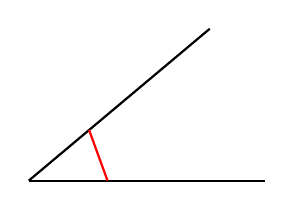
\begin{tikzpicture}
            \draw[thick] (0,0) -- (3,0);
            \draw[thick] (0,0) -- ({3*cos(40)},{3*sin(40)});
            \draw[red,thick] (1,0) -- ({cos(40)},{sin(40)});
        \end{tikzpicture}
        \caption{Unions of half-lines from the origin are not length minimizing.}
        \label{fig: non area minimizing cones}
\end{figure}

\begin{cor}\label{cor: dim(Sing(C)) <= n-7}
    If \(C \subset \R^{n+1}\) is an area minimizing \(n\)-dimensional cone, then \(\dim_\Haus(\Sing(C) \le n-7\).
\end{cor}
\begin{proof}
    Applying iteratively Theorem~\ref{thm: Federer reduction}, for every \(k \le \dim_\Haus(\Sing(C))\) we find an area-minimizing \((n-k)\)-cone \(C_k \subset \R^{n-k+1}\) with at least a singular point. But by Corollary~\ref{cor: every area minimizing cone is flat for n<8}, we know that we must stop before getting to \(\R^7\).
\end{proof}

\subsection{Existence of non-flat area minimizing cones}

In \cite{Simons_MinimalVarieties1968}, Simons introduced the famous \emph{Simons cone}
\[
    C_S \coloneq \{ (x,y) \in \R^4 \times \R^4 \colon |x|=|y|\} \subset \R^8,
\]
and he proved that it's stable (because the link is \(S=\Sp^3(1/\sqrt{2}) \times \Sp^3(1/\sqrt{2})\), and \(\mu_1(S)=-(n-1)=6\), so \(d_0(C)\ge 0\). One year later, Bombieri, De Giorgi and Giusti proved the following. 

\begin{thm}[Bombieri, De Giorgi, Giusti, {\cite{BombieriDeGiorgiGiusti_MinimalCones1969}}]\label{thm: C_S is area minimizing}
    \(\R^8 \setminus C_S\) is foliated by complete, smooth, area minimizing hypersurfaces \(\Sigma_\lambda\) (for \(\lambda \ne 0\)) which are invariant under the action of \(O(4)\times O(4)\) and such that \(\llbracket \Sigma_\lambda \rrbracket \weakstarto \llbracket C_S\rrbracket\) as \(\lambda \to 0\). In particular, \(C_S\) is area minimizing, and therefore \(C_S \times \R^{n-7} \subset \R^{n+1}\) is area minimizing for every \(n\ge 7\).
\end{thm}
